\documentclass[11pt]{article}

\usepackage[utf8]{inputenc} % character encoding - you don't need to understand this

% below are a bunch of useful packages, it doesn't cost anything to include them all so you might as well
\usepackage{amsmath}		% lets you input equations in math mode
\usepackage{graphicx}		% lets you include images
\usepackage{enumerate}		% lets you make lists
\usepackage{hyperref}		% lets you make links
\usepackage{subcaption}     % if you want to use subcaptions
\usepackage[all]{hypcap}	% makes links refer to figures and not captions
\usepackage{relsize}		% lets you use relative font sizes
\usepackage{caption}        % lets you add captions
\usepackage{array}          % lets you specify table column widths
\usepackage{siunitx}
\usepackage[margin=1in, paperwidth=8.5in, paperheight=11in]{geometry} % I'll bet you can figure this one out

% this line starts the actual document and text
\begin{document}

\title{ISIM Lab 3: An Analysis of the Humidity in Needham, MA, USA}
\author{Ari Porad}
% \date{date here} % leave this commented to display the current date
\maketitle % don't forget to include this line or you won't have a document header

\begin{abstract}
    A humidity transducer, which functions as a capacitor with a defined relationship between capacitance and relative humidity, was installed as the upper element in a voltage divider. The lower element of the voltage divider was a $10k\Omega$ resistor, and the input was an 10kHz square wave with a 0.5V amplitude centered at +0.5V. The circuit was calibrated by replacing the transducer with various capacitors of known capacitance, measuring the voltages, and calculating a line of best fit accordingly. This calibration line was then used to derive the capacitance of the humidity transducer from the measured voltage across it. From there, the calibration table provided in the transducer's data sheet was used to determine the actual measured humidity from the capacitance.
\end{abstract}

\section{Methodology}

\begin{figure} [H]
% the "!ht" will tell LaTeX to try and put the figure here, and at the top of the next page if it doesn't fit here. Getting figures to show up where you want can be a pain

	\centering  % this centers the image
	
	\includegraphics[width=0.75\textwidth]{circuit_diagram.jpg}
	% here I put the width as a fraction of the text width. You can also use a set number of inches, mm, pt, etc.
	% the text in the curly brackets is the name of the file. If it doesn't work, try adding the file extension, e.g. .jpg
	
	\captionsetup{margin={0.28\textwidth,0.28\textwidth}}
	% by adding margins to your caption, you can make the caption wrap with your figures rather than at the normal text width
	
	\caption{\smaller{Our measurement circuit. We connected the relative humidity transducer as the upper element in a voltage divider, with the lower element as a $10k\Omega$ resistor. The input to this voltage divider was the O-Scope's wave generator, while the output was to ground.}}
	% always caption your figures!
	
	\label{fig:circuit}
	% the label here allows me to reference this figure in text anywhere in this document. By matching the text inside the curly brackets of \label{} here and \ref{} in a paragraph, LaTeX automatically inserts the correct figure number and creates a link between the number and the referenced figure. As good practice, always use "fig:" at the beginning of figure labels
\end{figure}

A humidity transducer is a capacitor who's capacitance changes with a defined relationship to relative ambient humidity. We measured the capacitance of the circuit using a voltage divider, with the transducer as the upper element and a $10k\Omega$ resistor as the lower element, with the measurement leads of the O-Scope connected to either lead of the transducer. The input to the voltage divider was the O-Scope's wave generator, which was configured to produce a square wave of 0.5V amplitude, centered at 0.5V with a frequency of 10kHz (as prescribed by the transducer's data sheet). For comparison, the measurement leads of the other channel of the O-Scope were connected to the output of the wave generator and to ground. See Figure~\ref{fig:circuit}.

\begin{figure} [!ht]
% the "!ht" will tell LaTeX to try and put the figure here, and at the top of the next page if it doesn't fit here. Getting figures to show up where you want can be a pain

	\centering  % this centers the image
	
	\includegraphics[width=0.5\textwidth]{breadboard.jpg}
	% here I put the width as a fraction of the text width. You can also use a set number of inches, mm, pt, etc.
	% the text in the curly brackets is the name of the file. If it doesn't work, try adding the file extension, e.g. .jpg
	
	\captionsetup{margin={0.28\textwidth,0.28\textwidth}}
	% by adding margins to your caption, you can make the caption wrap with your figures rather than at the normal text width
	
	\caption{\smaller{Our breadboard, as used to measure the voltage across the transducer using a voltage divider.}}
	% always caption your figures!
	
	\label{fig:breadboard}
	% the label here allows me to reference this figure in text anywhere in this document. By matching the text inside the curly brackets of \label{} here and \ref{} in a paragraph, LaTeX automatically inserts the correct figure number and creates a link between the number and the referenced figure. As good practice, always use "fig:" at the beginning of figure labels
\end{figure}


\subsection{Calibration}

While our circuit directly measured voltage drop across the transducer, the transducer's data sheet provided humidity measurements in terms of capacitance. Consequently, we needed to determine the relationship between measured voltage across the transducer and capacitance. To do this, we replaced the transducer with several capacitors of known capacitance and measured the resulting voltage. We used this data to calculate a line of best fit between measured voltage and capacitance.

\section{Results}

\subsection{Calibration}

We calibrated our system using five capacitors, with the following known capacitances and measured voltages:

\begin{table}[H]
    \centering
    \begin{tabular}{ll}
    \hline
    \multicolumn{1}{c}{\textbf{Known Capacitance (pF)}} & \multicolumn{1}{c}{\textbf{Measured Voltage (mV)}} \\ \hline
    100pF &  84.8mV \\
    120pF & 102.7mV \\
    150pF & 118.4mV \\
    180pF & 123.5mV \\
    220pF & 150.4mV \\ \hline
    \end{tabular}
    \caption{\smaller{Measured voltages and known capacitances of our calibration capacitors.}}
    \label{table:calibration}
\end{table}

From this data, we calculated the following linear regression, which represents our system's relationship between measure voltage (V) and capacitance (pF). A visual comparison between our data and the regression can also be seen in Figure~\ref{fig:calibration}.

\begin{equation}
    \text{C} = 1.92V - 68.45
\end{equation}

\begin{figure}[H]
	\centering 
	\includegraphics[width=0.7\textwidth]{calibration.eps}
	\captionsetup{margin={0.2\textwidth,0.2\textwidth}}
	\caption{\smaller{Voltage vs. capacitance, showing our five calibration capacitors and our calculated calibration trend line. $R^2 = 0.97$}}
	\label{fig:calibration}
\end{figure}

\subsection{Humidity Measurement}

After calculating our calibration trend line, we reconnected the humidity transducer and measured the voltage across it. We then used the calibration trend line to calculate the capacitance of the transducer, and the transducer's data sheet to derive the measured humidity from its capacitance. The measured capacitance of the transducer was 171.13pF (see Figure~\ref{fig:results}). The actual relative humidity at the time (as provided by Weather.com) was 25\%. The data sheet of the transducer specifies that its capacitance will be 169.0pF at 20\% RH, 170.7pF at 25\% RH, and 172.3pF at 30\% RH, meaning that the closest value would be 25\% RH (exactly the same as the known humidity). While the precision of the data sheet doesn't permit a precise evaluation of the measurement's accuracy, it's safe to say that this system was highly accurate—especially considering that the humidity in the room may have deviated slightly from the measured humidity of all of Needham, MA, USA.

\begin{figure}[H]
	\centering 
	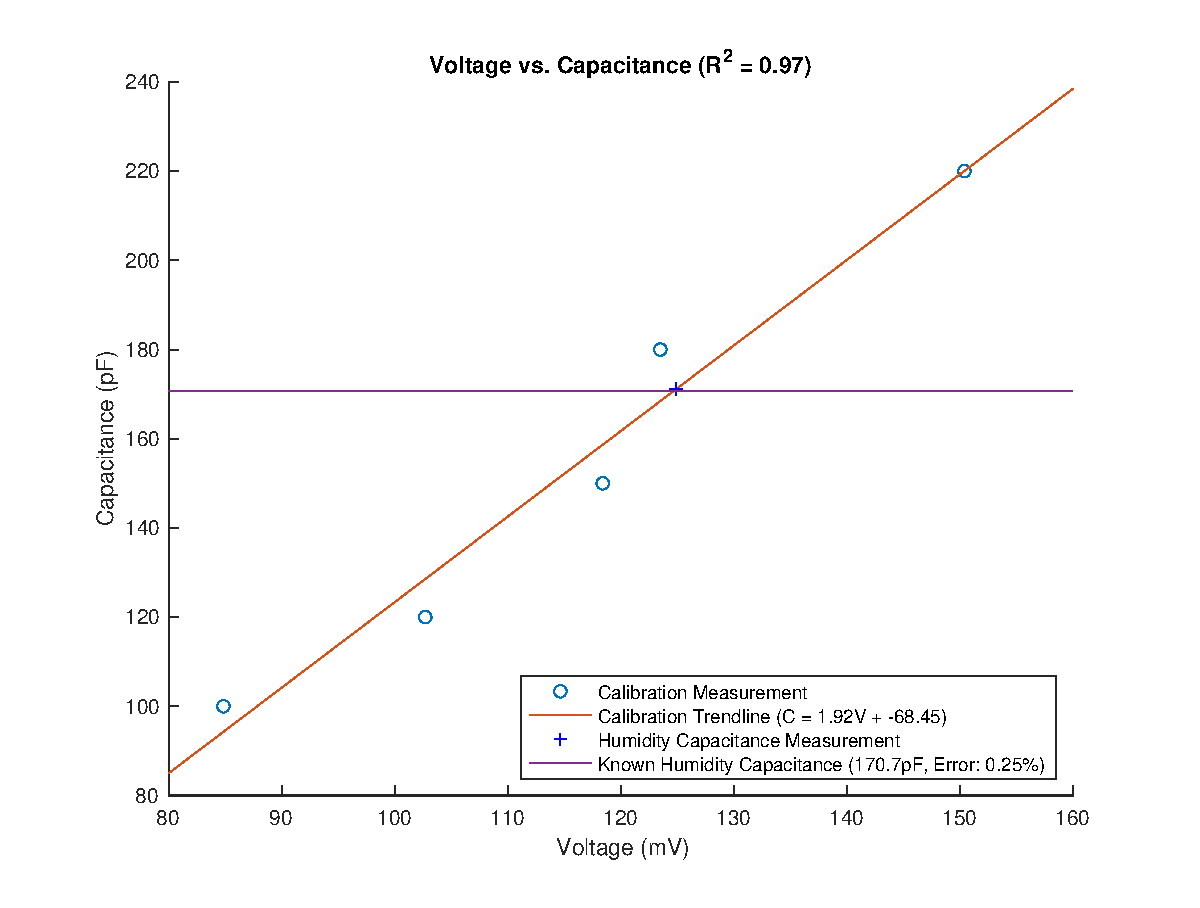
\includegraphics[width=0.7\textwidth]{full_results.eps}
	\captionsetup{margin={0.2\textwidth,0.2\textwidth}}
	\caption{\smaller{Voltage vs. capacitance, showing the humidity transducer's measured and true capacitance in addition to our calibration capacitors and our calculated calibration trend line.}}
	\label{fig:results}
\end{figure}


\subsection{CR Circuit vs. RC Circuit}

\begin{figure}[H]
	\centering 
	\includegraphics[width=0.7\textwidth]{voltage.eps}
	\captionsetup{margin={0.2\textwidth,0.2\textwidth}}
	\caption{\smaller{Voltage vs. time, showing the square wave produced by the O-Scope (blue) and the voltage across the transducer (orange)}}
	\label{fig:voltage}
\end{figure}

Because this circuit—unlike many of the circuits we've previously covered in class—is a CR circuit instead of an RC circuit, our system measures the voltage drop across the resistor instead of across the capacitor. As a result of this, the voltage across the transducer is shown to spike at the start of a wave cycle before immediately degrading. Half way through the cycle, when the voltage of the wave drops to 0, the voltage of the transducer again spikes in the negative direction, before degrading towards zero (Figure~\ref{fig:voltage}). This is the mirror image of what we'd expect for an RC circuit.

\section{Finishing Remarks}
This experiment demonstrated that a transducer is a highly accurate method for measuring relative humidity. More experimentation is required to test this system under a wider range of circumstances and with a higher degree of precision.
\end{document}